\section{Results}

% ── Worked Example ────────────────────────────────────────────────────
\begin{frame}{Example: Bulk Job Cancellation (End-to-End Trace)}
  \footnotesize
  \begin{columns}[T]
    \begin{column}{0.48\textwidth}
      \textbf{User prompt}\\
      \texttt{"Cancel all of charlie's running jobs"}\\[0.4em]
      \textbf{Observer (Think → Act → Observe)}\\
      \textit{Think:} User wants to cancel multiple jobs — state-changing, must hand off.\\
      \textit{Act:} \texttt{transfer\_to\_operator(\{action: "cancel", user: "charlie", scope: "all\_running"\})}\\[0.4em]
      \textbf{Operator}\\
      \textit{Discovery read:} \texttt{squeue(user="charlie")} → jobs \texttt{[3001, 3002, 3007]}\\
      \textit{Pending action created — awaiting HITL\ldots}\\[0.4em]
      \textbf{User:} ``Confirm''\\[0.4em]
      \textit{Execute:} \texttt{scancel(job\_ids=[3001,3002,3007])} \ding{51}\\
      \textit{Return to Observer} → final response.
    \end{column}
    \begin{column}{0.48\textwidth}
      \textbf{Evaluation scoring for this case}\\[0.3em]
      \renewcommand{\arraystretch}{1.2}
      \begin{tabular}{lcc}
        \toprule
        Dimension & Score & Weight \\
        \midrule
        Tool recall   & 1.00 & 0.35 \\
        Routing match & 1.00 & 0.25 \\
        HITL match    & 1.00 & 0.25 \\
        State match   & 1.00 & 0.15 \\
        \midrule
        \textbf{Overall} & \textbf{1.00} & — \\
        \bottomrule
      \end{tabular}\\[0.4em]
      Weighted score: $s = \mathbf{1.00}$ \ding{51}\\[0.4em]
      \textit{Key}: if agent skips HITL or uses wrong tool → lower weighted score.
    \end{column}
  \end{columns}
\end{frame}

% ── Three-Way Comparison ──────────────────────────────────────────────
\begin{frame}{Three-Way Model Comparison (615 Test Cases)}
  \centering
  \renewcommand{\arraystretch}{1.25}
  \begin{tabular}{lccc}
    \toprule
    \textbf{Metric} & \textbf{GPT-5-mini} & \textbf{FT Qwen (ours)} & \textbf{Base Qwen} \\
    \midrule
    Avg weighted score & 95.9\%  & \cellcolor{myNewColorC!20}\textbf{88.3\%}  & 85.2\%  \\
    Tool recall       & 98.8\%  & \cellcolor{myNewColorC!20}\textbf{89.2\%}  & 84.9\%  \\
    Routing match     & 99.0\%  & \cellcolor{myNewColorC!20}\textbf{90.1\%}  & 83.6\%  \\
    HITL match        & 99.0\%  & \cellcolor{myNewColorC!20}\textbf{90.4\%}  & 90.2\%  \\
    State match       & 98.2\%  & \cellcolor{myNewColorC!20}\textbf{90.0\%}  & 89.8\%  \\
    Judge score       & 75.7\%  & \cellcolor{myNewColorC!20}\textbf{79.7\%}  & 76.8\%  \\
    Avg latency       & 28.3\,s & \cellcolor{myNewColorC!20}84.8\,s & 80.9\,s \\
    \bottomrule
  \end{tabular}\\[0.5em]
  \small All three systems run the Observer/Operator dual-agent architecture on the same 615-case held-out test set.
  \vspace{0.4em}
  \begin{itemize}
    \item FT Qwen closes \textbf{29\% of the gap} to GPT-5-mini
    \item Judge score \textbf{exceeds} both base (76.8\%) and commercial (75.7\%)
    \item Local deployment: no API cost, no data transmission
  \end{itemize}
\end{frame}

% ── Per-Category ──────────────────────────────────────────────────────
\begin{frame}{Per-Category Average Scores: Three-Way Comparison}
  \centering
  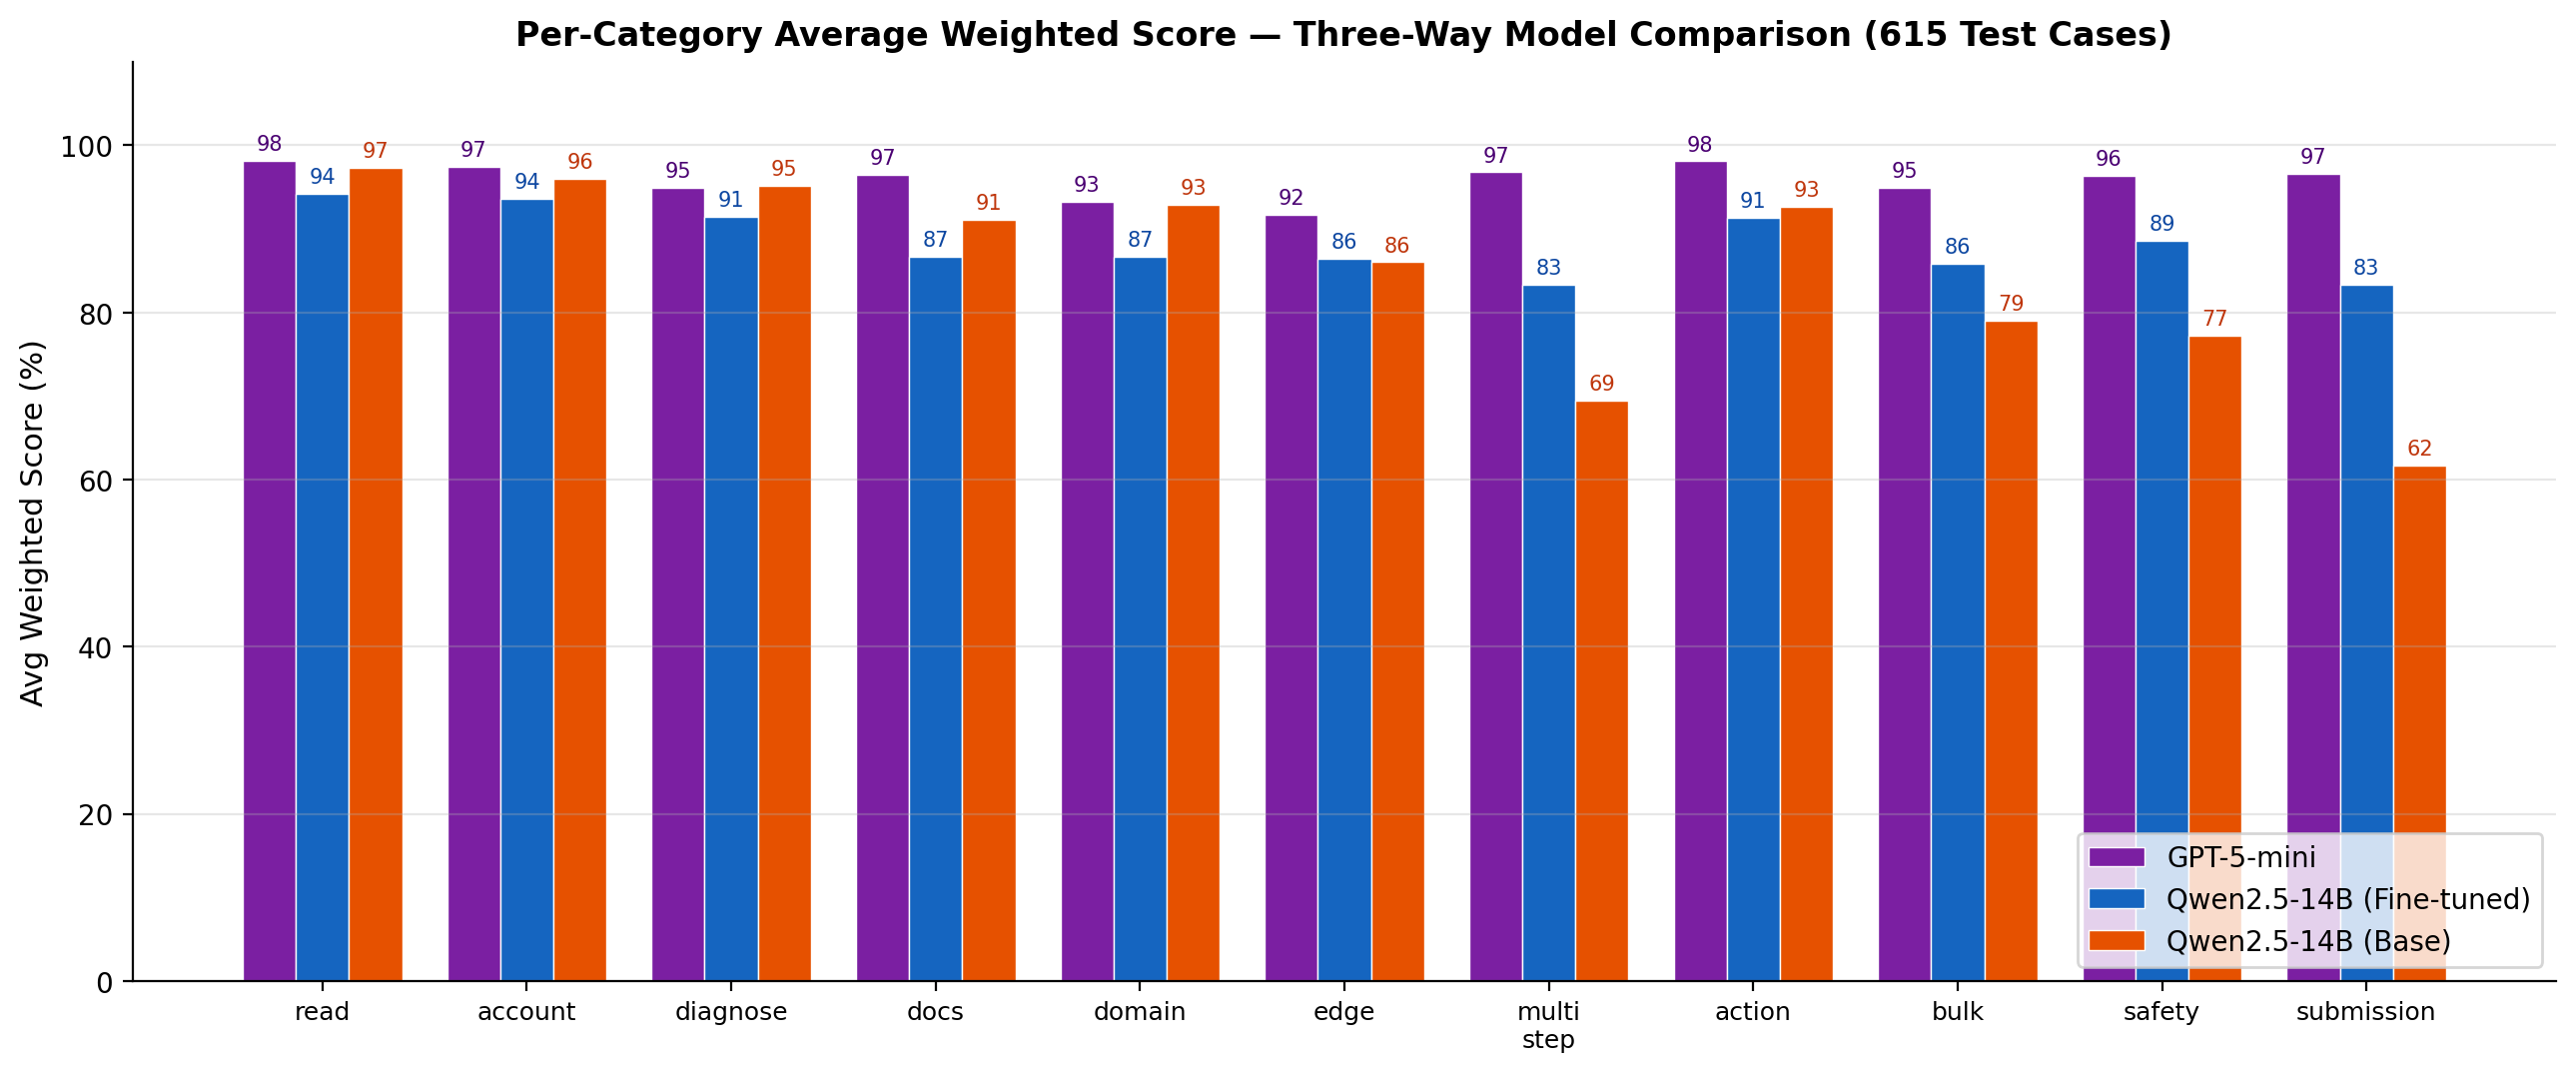
\includegraphics[width=0.96\textwidth]{../report/images/evaluation/three_way_per_category.png}
  \captionof{figure}{GPT-5-mini (purple) vs.\ FT Qwen (blue) vs.\ Base Qwen (orange). Largest FT gains: submission $+$21.7\,pp, multi\_step $+$13.8\,pp, safety $+$11.3\,pp, bulk $+$6.8\,pp}
\end{frame}

% ── Architecture Ablation ─────────────────────────────────────────────
\begin{frame}{Architecture Ablation: Dual-Agent vs.\ Monolithic}
  \begin{columns}[T]
    \begin{column}{0.50\textwidth}
      \renewcommand{\arraystretch}{1.2}
      \small
      \begin{tabular}{lccc}
        \toprule
        \textbf{Metric} & \textbf{O/O} & \textbf{Mono} & \textbf{$\Delta$} \\
        \midrule
        Avg $s_{\text{abl}}$ & 87.6\% & 81.6\% & +6.1\,pp \\
        Tool recall    & 84.9\% & 77.5\% & +7.4\,pp \\
        HITL match     & 90.2\% & 88.9\% & +1.3\,pp \\
        State match    & 89.8\% & 78.9\% & +10.9\,pp \\
        Judge score    & 76.8\% & 59.2\% & +17.6\,pp \\
        \bottomrule
      \end{tabular}
      \vspace{0.3em}\\
      \tiny Both scored with $s_{\text{abl}}$ (see Scoring Methodology slide)
    \end{column}
    \begin{column}{0.46\textwidth}
      \textbf{What the ablation shows}
      \begin{itemize}
        \item +6.1\,pp on same base model, same formula — pure architecture gain
        \item \textbf{Safety}: Observer structurally cannot call \texttt{scancel}
        \item \textbf{Tool scope}: +7.4\,pp tool recall from halved catalog
        \item 378 routing-neutral cases: +10.2\,pp
      \end{itemize}
    \end{column}
  \end{columns}
\end{frame}

% ── Ablation Per Category ─────────────────────────────────────────────
\begin{frame}{Ablation: Per-Category Average Score}
  \centering
  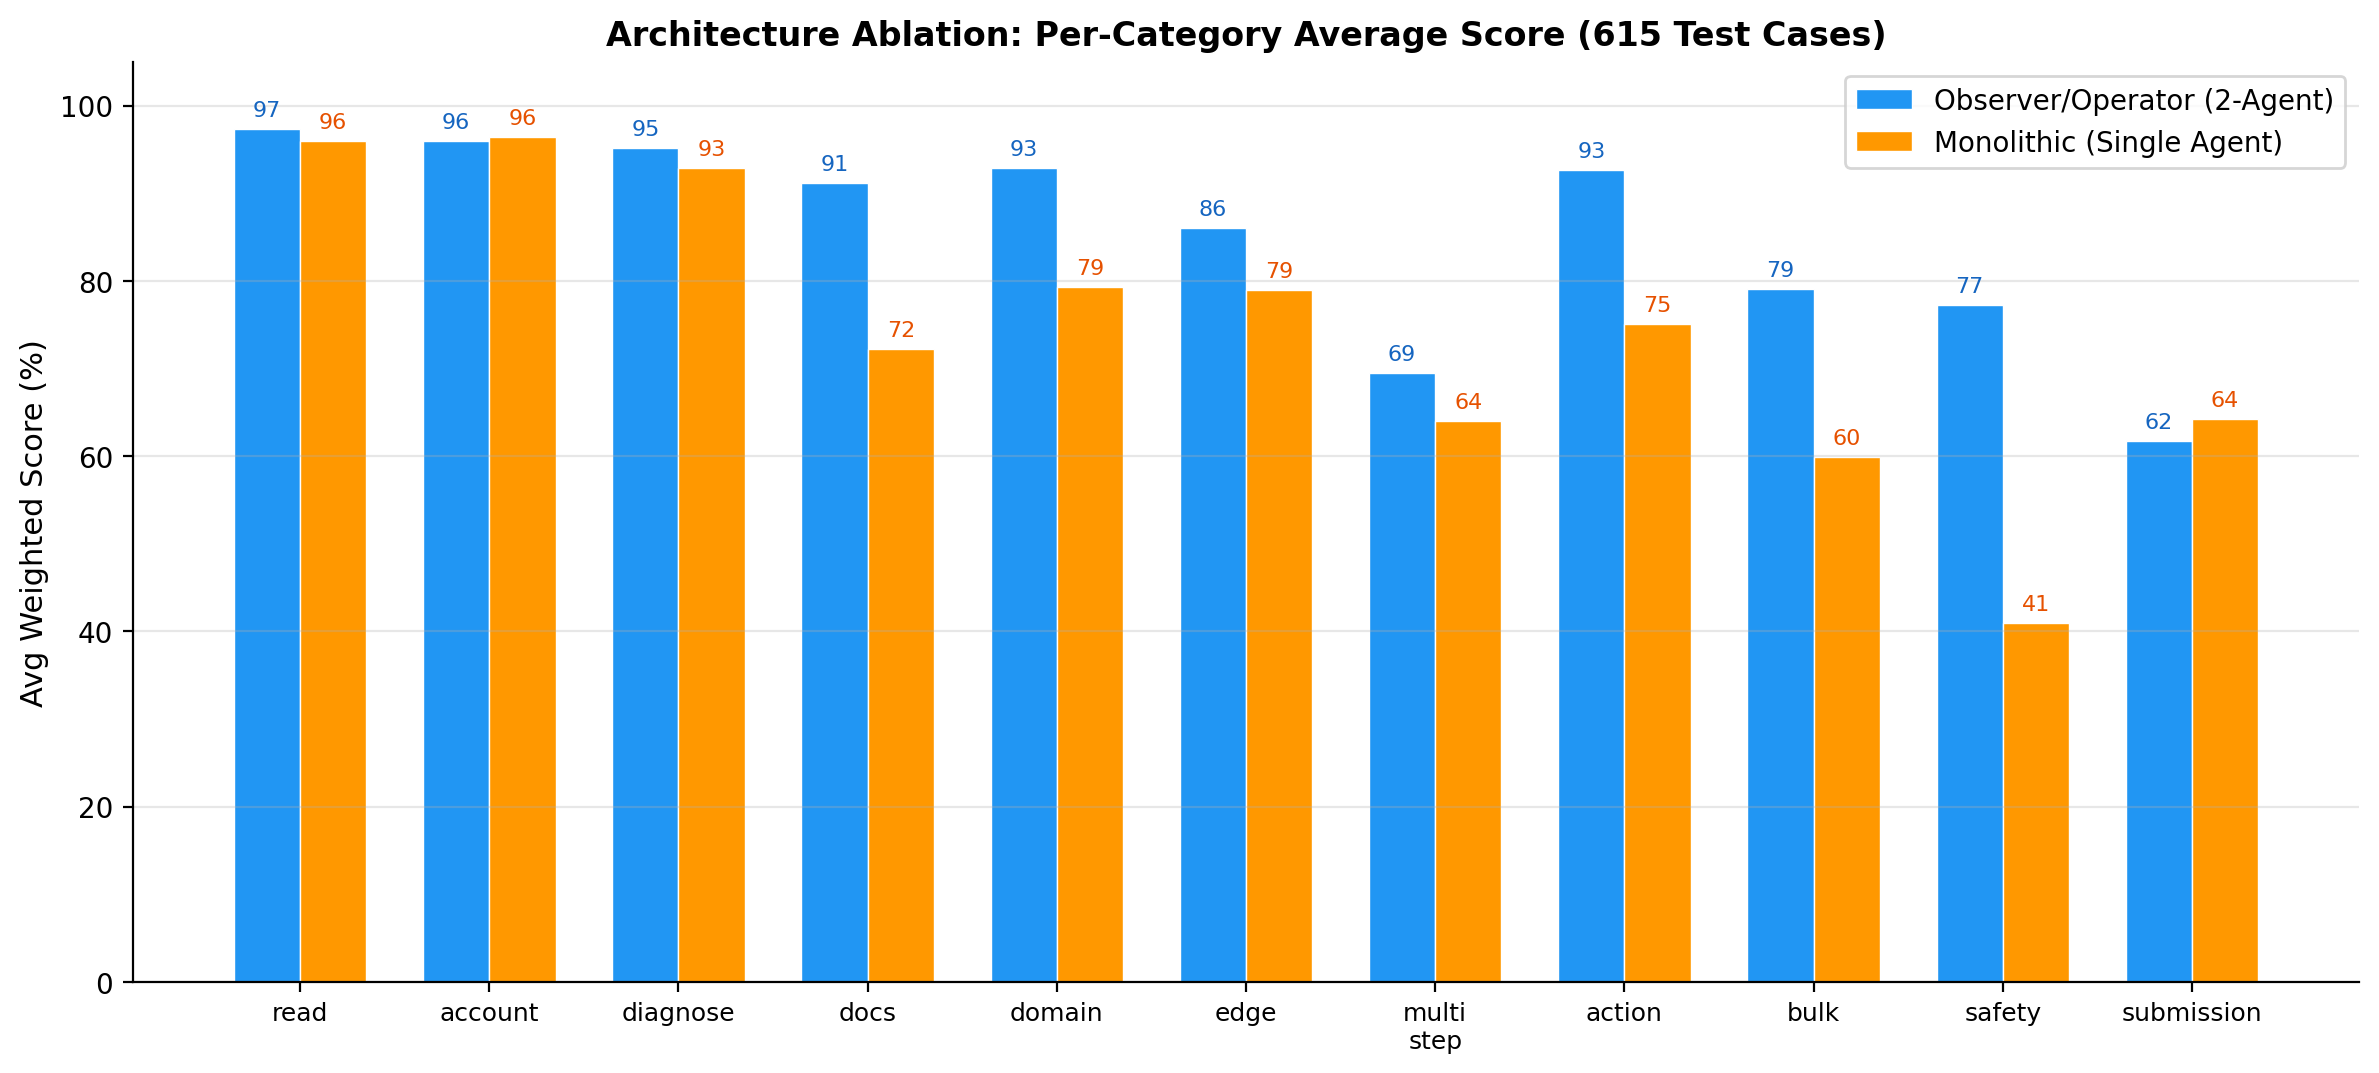
\includegraphics[width=0.95\textwidth]{../report/images/evaluation/ablation_per_category.png}
  \captionof{figure}{Observer/Operator vs.\ Monolithic per category. Action/bulk/safety categories collapse without the Operator confirmation gate.}
\end{frame}

% ── UI Demo ───────────────────────────────────────────────────────────
\begin{frame}{System Demo — HITL Confirmation (Before)}
  \centering
  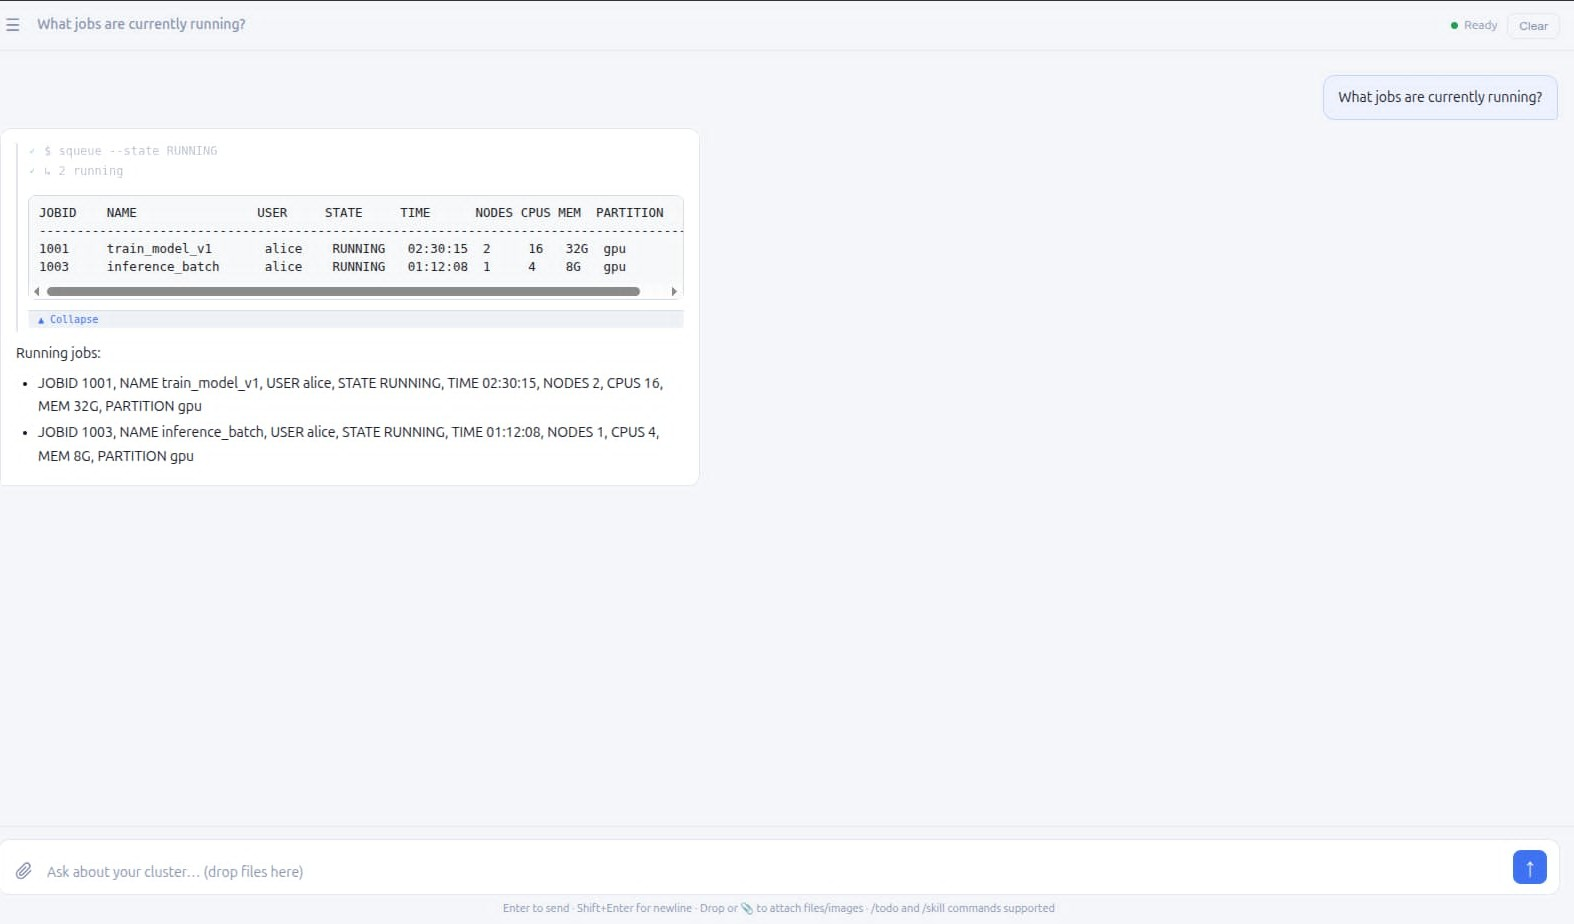
\includegraphics[height=0.82\textheight]{../report/images/UI_before_HITL.jpg}
  \captionof{figure}{User requests a destructive action; Observer routes to Operator for confirmation.}
\end{frame}

\begin{frame}{System Demo — HITL Confirmation (During)}
  \centering
  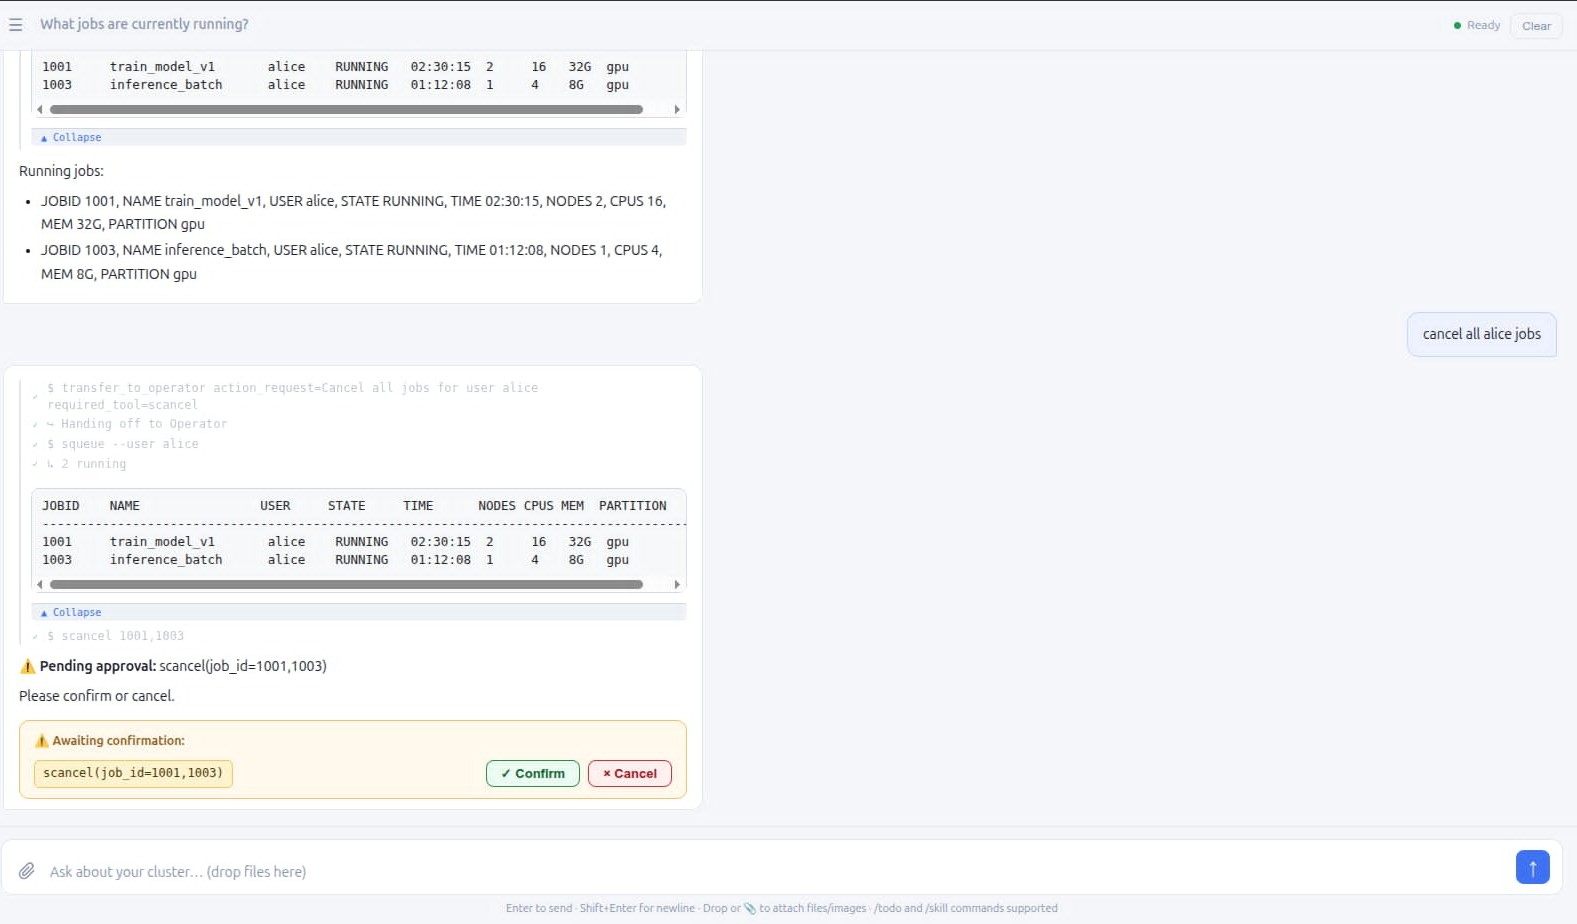
\includegraphics[height=0.82\textheight]{../report/images/UI_during_HITL.jpg}
  \captionof{figure}{HITL confirmation gate — pending action awaiting user approval.}
\end{frame}

\begin{frame}{System Demo — HITL Confirmation (After)}
  \centering
  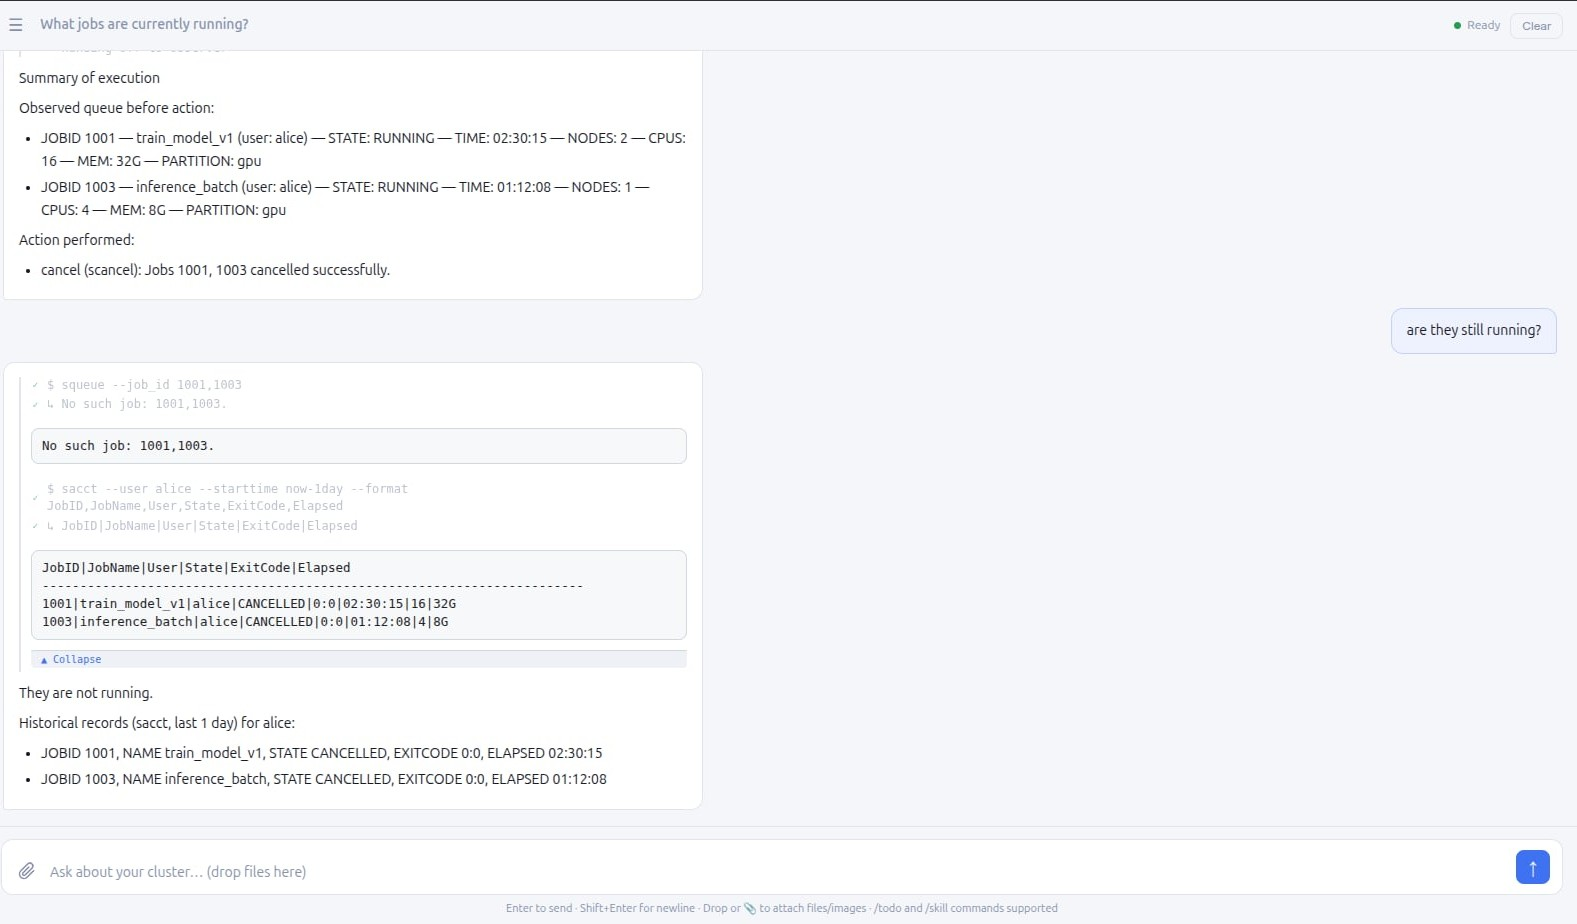
\includegraphics[height=0.82\textheight]{../report/images/UI_after_HITL.jpg}
  \captionof{figure}{After approval: confirmed execution with result summary.}
\end{frame}

\begin{frame}{System Demo — RAG Documentation (Before)}
  \centering
  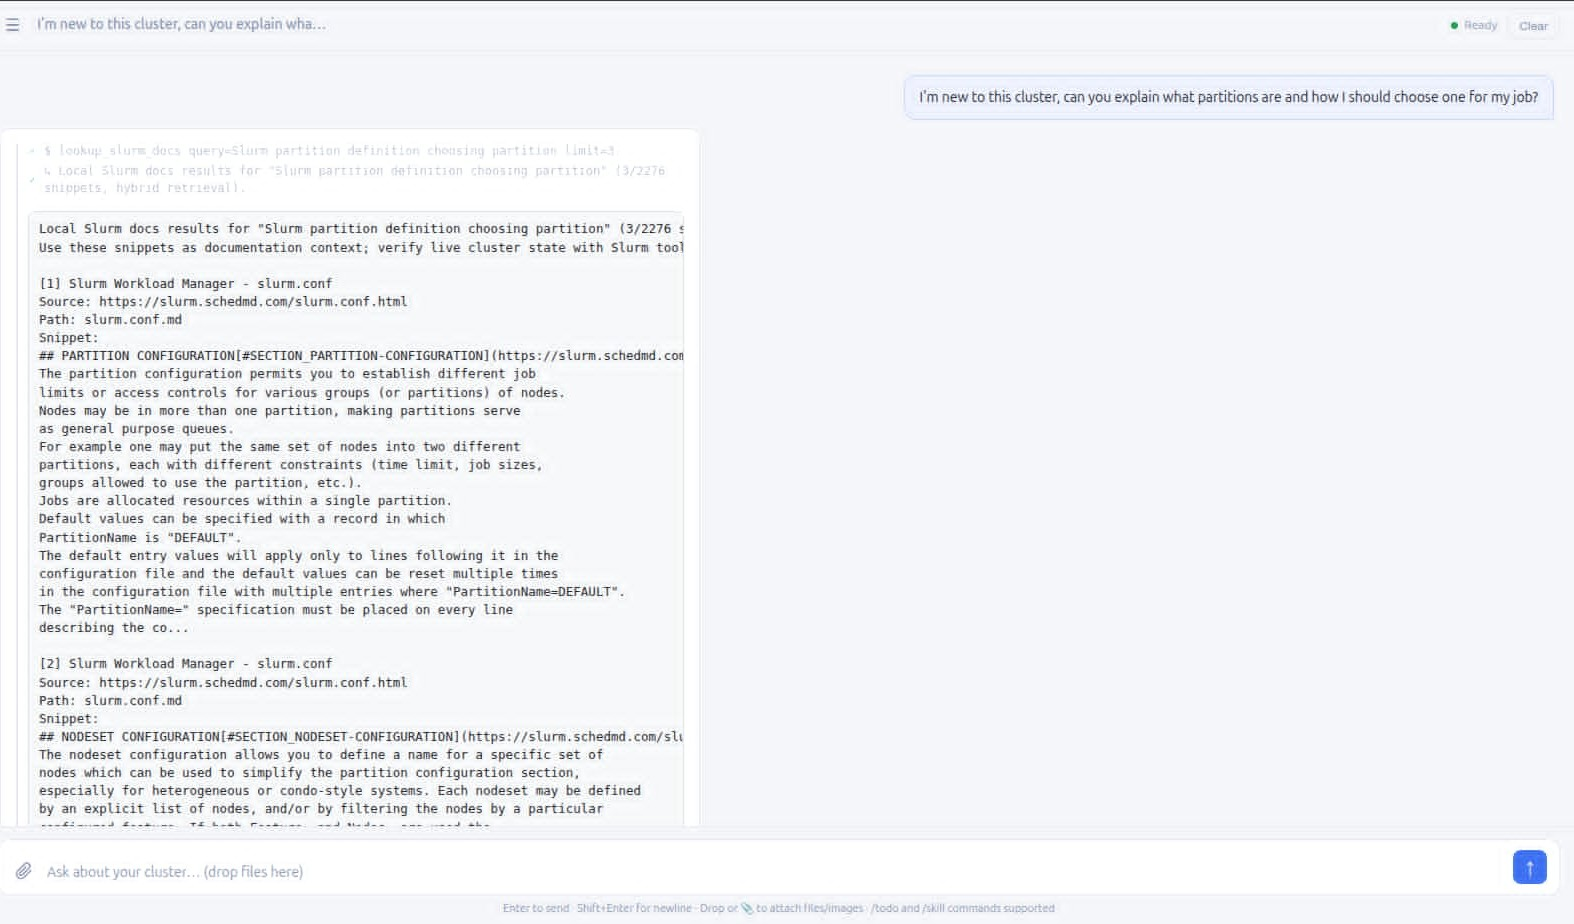
\includegraphics[height=0.82\textheight]{../report/images/UI_before_RAG.jpg}
  \captionof{figure}{User asks a Slurm documentation question.}
\end{frame}

\begin{frame}{System Demo — RAG Documentation (After)}
  \centering
  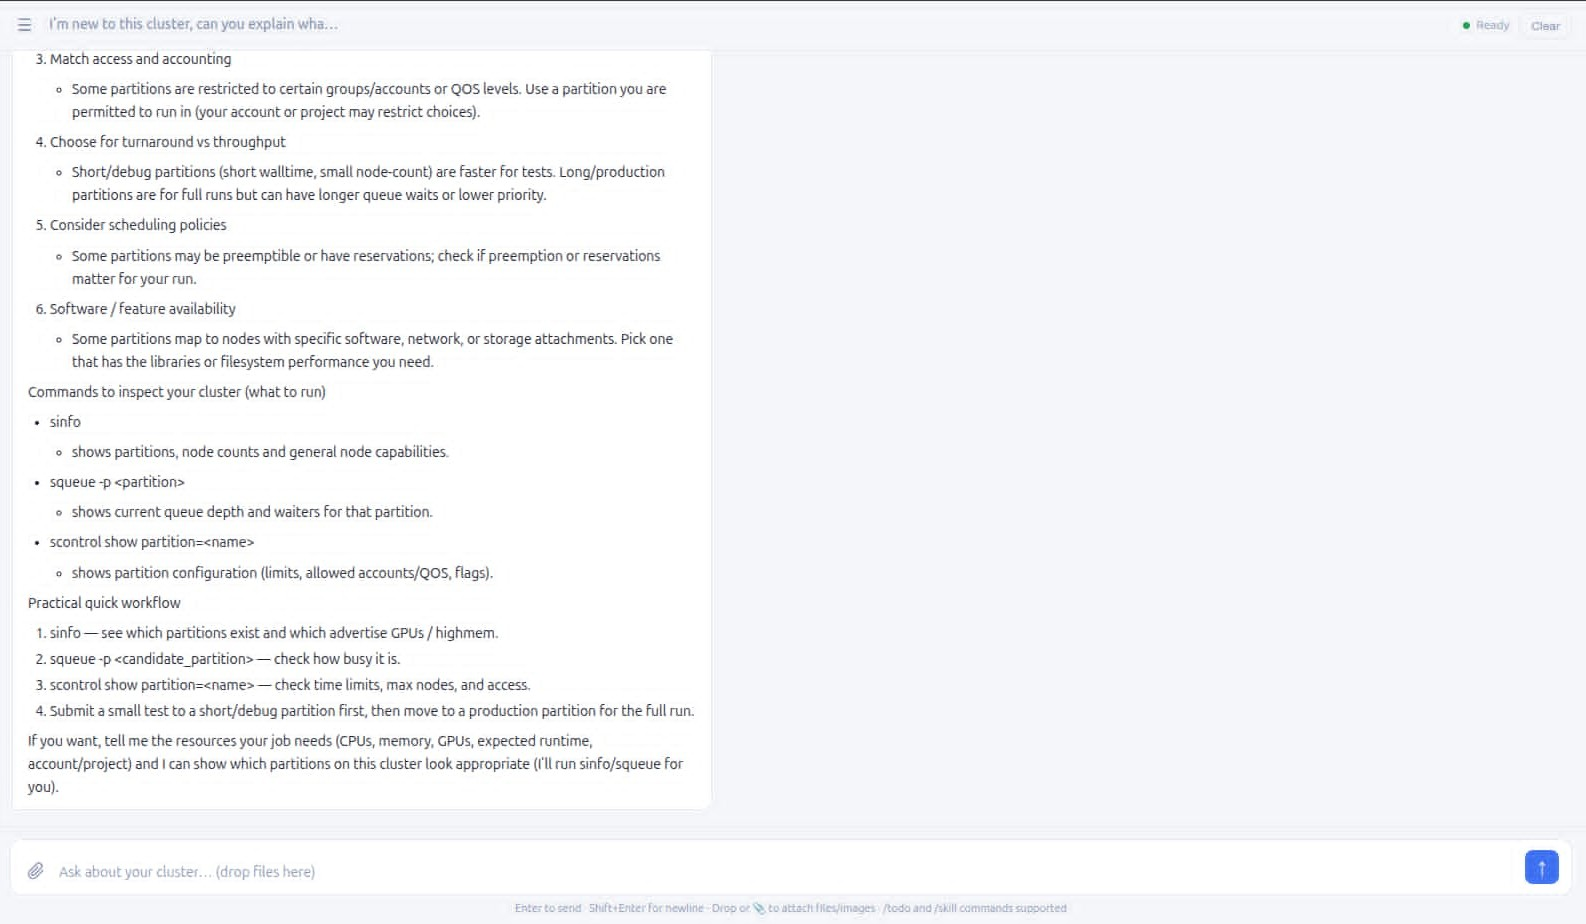
\includegraphics[height=0.82\textheight]{../report/images/UI_after_RAG.jpg}
  \captionof{figure}{Agent retrieves and synthesizes relevant documentation via RAG tools.}
\end{frame}

\begin{frame}{System Demo — Web Search (Before)}
  \centering
  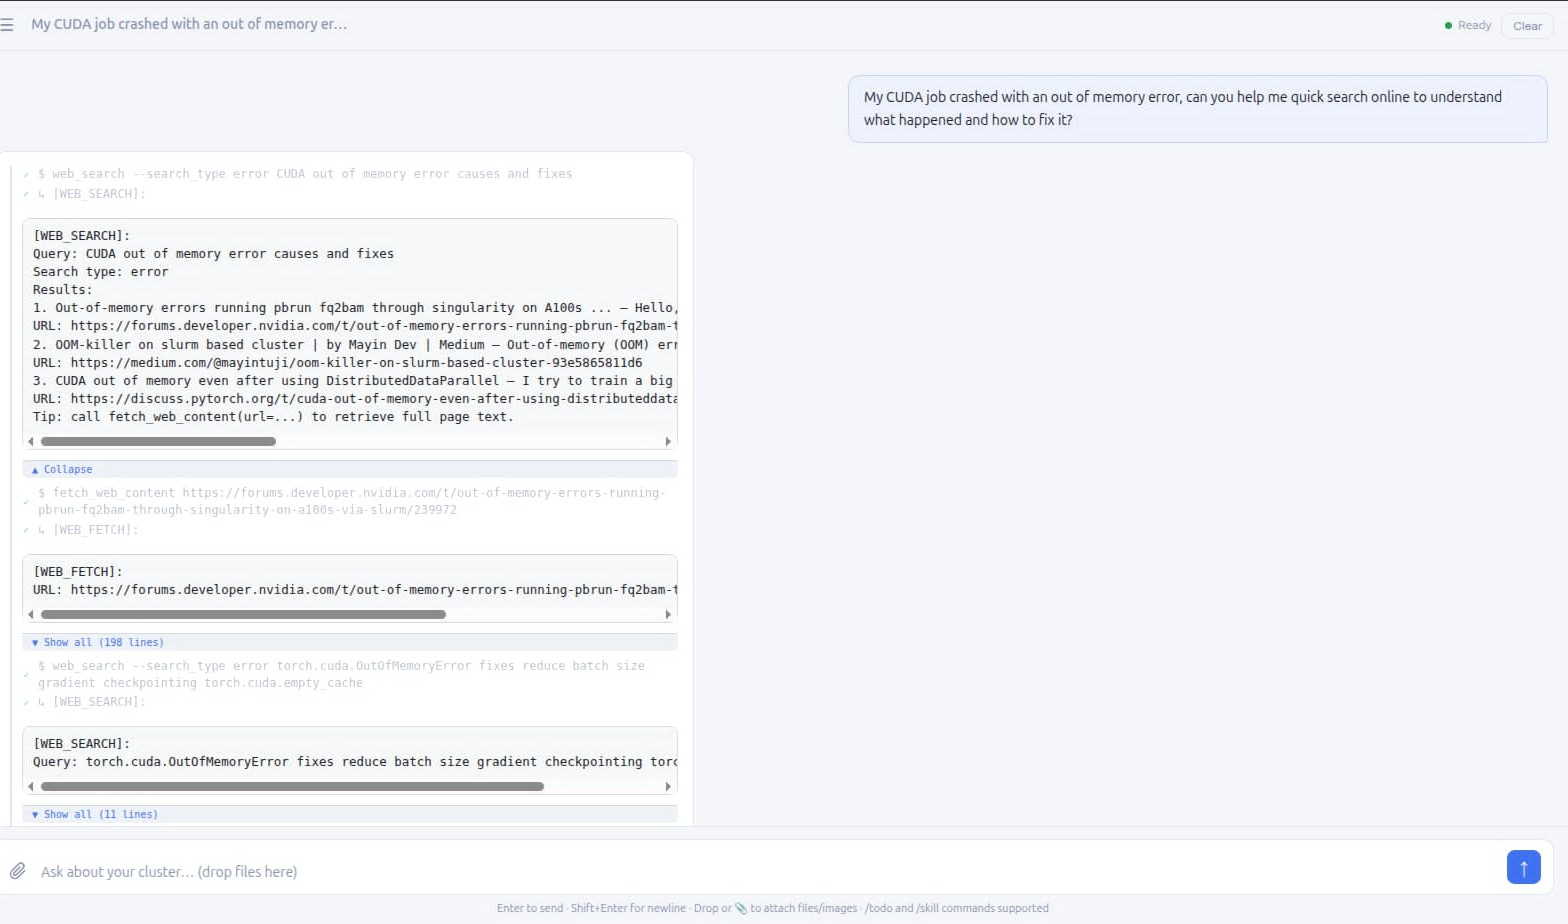
\includegraphics[height=0.82\textheight]{../report/images/UI_before_WEB.jpg}
  \captionof{figure}{User asks a question requiring external knowledge.}
\end{frame}

\begin{frame}{System Demo — Web Search (After)}
  \centering
  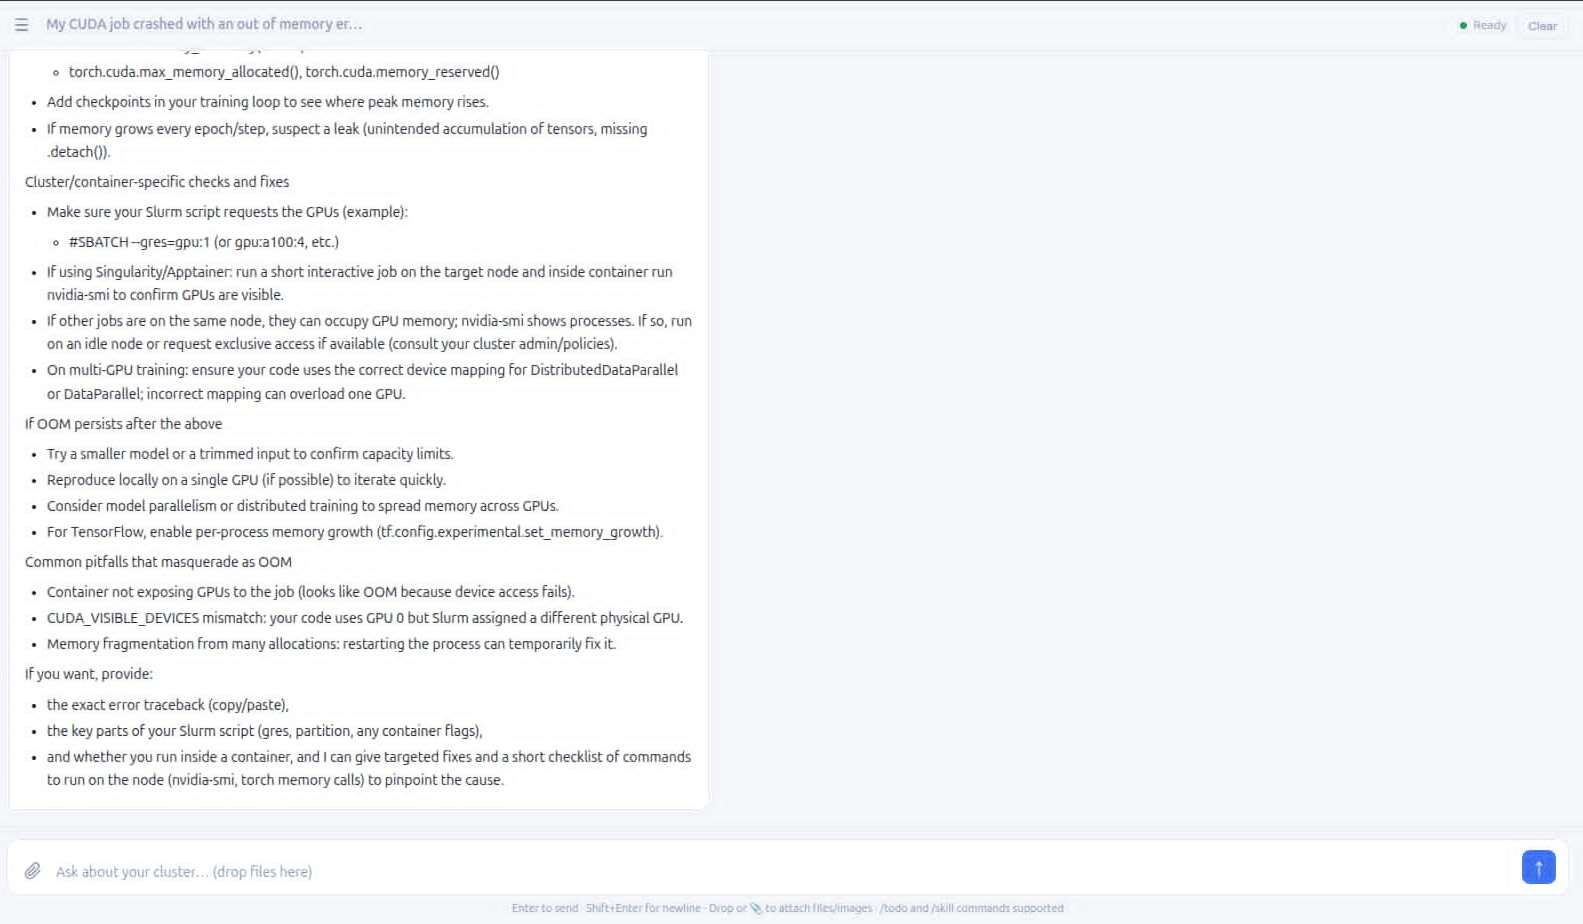
\includegraphics[height=0.82\textheight]{../report/images/UI_after_WEB.jpg}
  \captionof{figure}{Agent performs web search and returns a cited answer.}
\end{frame}
